\chapter{Deployment}

\begin{chapterabstract}
    Example deployment, configuration and customization of the application. Examination of associated costs and the impact on business processes.
\end{chapterabstract}

In the following chapter, the attention is shifted from the development process to the deployment of the created solution. In this chapter, the focus is two-fold: firstly, the deployment of the solution is described in practical steps from the toolkit's administrator perspective, then business implications such as cost and process optimization are examined.

The setup of the solution is described from the point of view of a business wanting to utilize the tool. For illustration purposes, an example company is used in this chapter. The chosen company manufactures modular point-of-sale cardboard displays. To offer their product, they maintain a basic online presence using a simple WordPress website with information about the company, a showcase of their products, and an inquiry form which allows them to be contacted by their customer. In this scenario, the company aims to integrate the 3D configurator into its existing website to offer an interactive, user-friendly service that allows customers to customize and visualize options for their own configurations of cardboard displays.

By the end of this chapter, a comprehensive understanding of the deployment process of the toolkit from both a technical and business perspective will be provided.


%______________________________________________________________
\section{Application Setup and Configuration}
%______________________________________________________________

This section describes the necessary steps to utilize the implemented solution, from the perspective of a person designated by the business to operate the toolkit.


% - - - - - - - - - - - - - - - - - - - - - - - - - - - - - - -
\subsection{Building and Launching the Application}
% - - - - - - - - - - - - - - - - - - - - - - - - - - - - - - -

If the code of the application has been modified in any way, the installation of Node.js and npm is a prerequisite for building the application. The configurator application can then be built by executing \mintinline[bgcolor=backgroundgray]{bash}{npm install} followed by \mintinline[bgcolor=backgroundgray]{bash}{npm run build --workspace main}, which will generate the files in \texttt{apps/main/dist/} directory. If no modifications have been made, pre-built files may be utilized directly.

In the example case, the company already operates a website; therefore, the newly implemented configurator tool will be deployed to the appropriate subdomain of the website (e.g. \texttt{configurator.example.com}). This approach requires proper configuration of DNS settings for the new subdomain and appropriate adjustments to the web server, but otherwise utilizes the already existing web hosting infrastructure. If this were not the case, it would be necessary to facilitate an HTTP server through web hosting.

To deploy the application, the built files need to be copied to the web server, ensuring that they are statically served. The \texttt{index.html} file loads and initializes that application on access.

Due to the implementation of client-side routing, the web server needs to be adjusted to correctly redirect requests. A web server by default interprets request as a query for files located on the URL address, and since the routes defined in the application do not correspond to the actual files, the \textquote{not found} responses would be returned. Therefore, the server needs to be configured in such a way, that requests for nonexistent files are redirected to the \texttt{index.html} file, where they will be managed internally by React-Router. The company in the example case uses Apache HTTP Server, therefore its configuration \texttt{.httaccess} file, which sets the rules such that requests for nonexistent files, directories, or symlinks are redirected to \texttt{index.html} can be previewed in \autoref{listing:apache-config}. A similar setup can be achieved in comparable fashion with NGINX or other web servers.

\begin{listing}[h]
\begin{minted}{text}
RewriteEngine On
 
RewriteCond %{REQUEST_FILENAME} !-f
RewriteCond %{REQUEST_FILENAME} !-d
RewriteCond %{REQUEST_FILENAME} !-l
 
RewriteRule ^ index.html [L]
\end{minted}
\caption{Configuration of Apache HTTP Server client-side routing with React-Router}
\label{listing:apache-config}
\end{listing}

With this set, the application should be functional and available, albeit yet without the content of configurable products.


% - - - - - - - - - - - - - - - - - - - - - - - - - - - - - - -
\subsection{Customizing the Application}
% - - - - - - - - - - - - - - - - - - - - - - - - - - - - - - -

The following section describes the adaptation of the deployed application to meet the needs and correspond to the identity of the business. This is done by the administrator through modifications of the \texttt{appconfig.json} file.


%______________________________________________________________
\subsubsection{Localizations}

To adjust the interface texts and provide different localization options, translation files should be created in the \texttt{locales/} directory. This functionality is described in more detail in \autoref{section:impl-languages}. These translations can be based on the English translation file included with the built application. Once the necessary language files are set up (note that supporting English is optional), they should be listed by their two-letter codes in the \texttt{appconfig.json} file under the \texttt{ui.languages.all} key. Additionally, a default language must be specified in \texttt{ui.languages.default}.


%______________________________________________________________
\subsubsection{Appearance}

Following, the appearance of the interface can be tailored. Color scheme is customizable by updating the hex color codes in \texttt{ui.colors} and for the outlines within the 3D preview in \texttt{spatialUi.selectionColors}. The logo displayed on the top left, as well as the favicon can be customized by setting the paths to the image files under \texttt{images} key. The web page to which the displayed logo links to can be configured using the \texttt{sources.homepageUrl} key. In addition, the title of the web page can be adjusted using the \texttt{title} key. The appearance customizations provide options for both dark and light modes of the interface.

Moreover, the camera style and floor shadow in the 3D visualization can be adjusted, and the option whether to display the button to save the completed configuration in PDF to users is provided.


%______________________________________________________________
\subsubsection{Data Source}

Finally, the source from which the product catalog is fetched must be defined in \texttt{sources.catalogUrl}. Any accessible location which provides the files in the correct data scheme can be provided here. Creation of this catalog file is described in the following section.


%______________________________________________________________
\subsubsection{Example Case}

In the example case discussed in this chapter, the interface was customized according to the company's brand guidelines. The company logo, set to appear in the top left corner, links back to the company's original website. The catalog source was defined as a static file located on the web server at \texttt{products/catalog.json}.


% - - - - - - - - - - - - - - - - - - - - - - - - - - - - - - -
\subsection{Catalog Creation and Content Management}
% - - - - - - - - - - - - - - - - - - - - - - - - - - - - - - -


The following section describes the process of managing configurable products for the deployed application.

The first step needed to create catalog of product is the preparation of 3D models that will be used in the configurator. The supported format is GLTF and its binary form GLB, to which other 3D formats can be converted. These files can be generated out of the CAD files used by the company to manufacture the products, or modeled manually. The images of the components that help the models with the representation should also be prepared and kept somewhere accessible.

It is necessary to store the files in an accessible location so that they can be fetched from their paths by the configurator application. It should be kept in mind that the size of the file and the complexity of the models correspond to the performance of the configurator application; therefore, it is beneficial to have simplified models with compressed textures to achieve the greatest possible performance. For easier of specification creation, the center of the model should also align with the center of the 3D scene in the file.

To create the configurable products, the administrative application needs to be launched. With the same prerequisites and dependencies as the main application, the admin tool can be built using the following command: \linebreak\mintinline[bgcolor=backgroundgray]{bash}{npm run build --workspace admin}

The resulting files will be created in \texttt{apps/admin/dist}. These built files can be again uploaded to a web server (perhaps within the company intranet) or be served locally for the duration needed to create the specifications by executing the command: \mintinline[bgcolor=backgroundgray]{bash}{npm run preview --workspace admin}

Within the administrator's application Product Composer screen, product specification can be now created, by creating component specifications along with their materials, mounting points and specified base components. It should be kept in mind that the 3D models of the components (and images) in the admin application are loaded from the same paths as they will be in the main application during configuration, and it is therefore crucial for these models to be accessible in both applications on the same paths. When product specifications are created, they can each be exported to JSON files, and again, need to be stored in accessible locations from the main application.

The catalog is then created in the Catalog Composer screen of the admin application. Each catalog entry must reference the location accessible from the main application where the product specification file created in the previous step can be fetched from. After the catalog is complete, it should be exported and stored at the location specified in the global config file, which was discussed in previous section.

For updates of the created specifications, the existing files can be downloaded, updated, imported back into the admin tool, edited, and then uploaded back to their original locations.

In the example company followed in this chapter, the 3D models were generated from CAD software used in manufacturing process of the company and stored as static files on the web server. Then, the admin application was utilized to create the product specifications and catalog, The created files were also transferred to the web server, from where they will be statically served. Given that the company utilizes an inquiry form on their website, the configurable products followed the same approach and had an inquiry form set as a confirmation action. A serverless function, hosted on Cloudflare Workers\footnote{\url{https://workers.cloudflare.com}}, was created to process the data. The function accepts the POST requests with the contact info and configuration created by the user sent from the inquiry form within the main application, and forwards these data to a company email. To enable this, the URL of this serverless function was set as the endpoint of the confirmation action in the Catalog Composer screen. A simplified illustration of the implementation of serverless functions can be seen in \autoref{listing:serverless}.

\begin{listing}[h!]
\begin{minted}{typescript}
async function handleRequest(request: Request) {
  const headers = new Headers({
    "Access-Control-Allow-Origin": "configurator.example.com",
    "Access-Control-Allow-Methods": "POST, OPTIONS",
    "Access-Control-Allow-Headers": "Content-Type"
  });

  if (request.method === "OPTIONS") {
    return new Response(null,
        { headers, status: 204 });
  }
  if (request.method !== "POST") {
    return new Response("Method Not Allowed",
        { headers, status: 405 });
  }

  const formData = await request.json();
  try {
    const parsedData = RequestSchema.parse(formData);
    await sendEmail(parsedData);
    return new Response(null, 
        { headers, status: 200 });
  } catch (error) {
    return new Response("Invalid data",
        { headers, status: 400 });
  }
}

addEventListener("fetch", event => {
  event.respondWith(handleRequest(event.request));
});
\end{minted}
\caption{Implementation of serverless function for forwarding inquiry form data}
\label{listing:serverless}
\end{listing}


%______________________________________________________________
\section{Business Aspects}
%______________________________________________________________

This section explores the business aspects of deploying the configurator tool, examining the cost effectiveness as well as business process modifications within the company.


% - - - - - - - - - - - - - - - - - - - - - - - - - - - - - - 
\subsection{Cost-Effectiveness}
% - - - - - - - - - - - - - - - - - - - - - - - - - - - - - - 

As this solution aims to cater to small businesses, this project has been conceptualized with cost effectiveness in mind, with the requirement of lightweight infrastructure needs (\hyperref[itm:NF4]{NF4}) and self-hostability (\hyperref[itm:NF3]{NF3}). These principles have been greatly reflected in the design and implementation.

The primary costs of this solution stem from the setting up of the tool, which includes acquiring 3D models and specifying the configurable content, as well as the customization of the tool and integration into the infrastructure. These costs can vary greatly between different companies, as some may be disposing of the necessary files, while others will have to create them. The complexity of the offered products that are defined in the tool also plays a role in this step.

From a technical standpoint, the infrastructure costs are low. For companies with an existing web server, no additional infrastructure is required. In addition, the costs of web hosting are minimal, as static websites can often be hosted free on platforms such as Cloudflare Pages \cite{CloudflarePages} or Netlify \cite{Netlify}. 

For functionalities the require additional processing of the product data or the inquiry form, serverless functions, as demonstrated in the previous case, can be used. Unless a very large amount of requests is processed, these can also be very cost-effective, and the summary of the pricing per requests for three major serverless providers (Cloudflare Workers, AWS Lambda, Google Cloud Functions) as of April 2024 can be seen in \autoref{table:lambda-price}.

\begin{table}[htb]
\centering
\begin{tabular}{>{\raggedright\arraybackslash}p{4.1cm} >{\raggedright\arraybackslash}p{4cm} >{\centering\arraybackslash}p{3.3cm}}
\toprule
\textbf{Provider} & \textbf{Free plan limits} & \multrow{c}{\textbf{Cost over limit} \\ \textbf{(per million reqs)}}\\ 
\midrule
Cloudflare Workers & 100 000 reqs/day & \$0,15 \\
AWS Lambda & 1 000 000 reqs/month & \$0,20 \\
Google Cloud Functions & 2 000 000 reqs/month & \$0,40 \\
\bottomrule
\end{tabular}
\captionsource{Overview of the pricing per requests (reqs) for serverless providers}{Cloudflare \cite{CloudflareWorkers}, Amazon \cite{AWS}, Google \cite{GoogleCloud}}
\label{table:lambda-price}
\end{table}


In the example company described in this chapter, the only expense associated with the tool was the time spent preparing the content and deploying the application.


%______________________________________________________________
\subsubsection{Return on Investment}

Consequently, the return on investment (ROI) for this solution is therefore projected to be hugely positive. While having minimal costs, the configurator not only acts as a sales assistance tool, allowing for detailed product visualization and customization, but also serves as a marketing tool that can enhance the company's market presence and appeal to a technically adequate consumer base. 


% - - - - - - - - - - - - - - - - - - - - - - - - - - - - - - 
\subsection{Operational Impact}
% - - - - - - - - - - - - - - - - - - - - - - - - - - - - - - 

Evaulating the impact deployment of the solution brings to businesses and companies is a complex task. The toolkit is adaptable and product-agnostic, meaning it can be utilized by different companies across different industries or in different parts of a supply chain. Consequently, the impact on processes will differ in each scenario.

Therefore, this section will describe the change in processes after the tool's deployment in the example company examined in this chapter, as this should serve as an illustration of one of the common effects this tool can have.

This solution deployed in the example company impacts the inquiry and order process. This section will describe this process before and after implementation. The process involves two actors: the customer wanting to purchase a product and the company employee handling the customer's requests.

\begin{landscape}
\begin{figure}[h!]
\centering
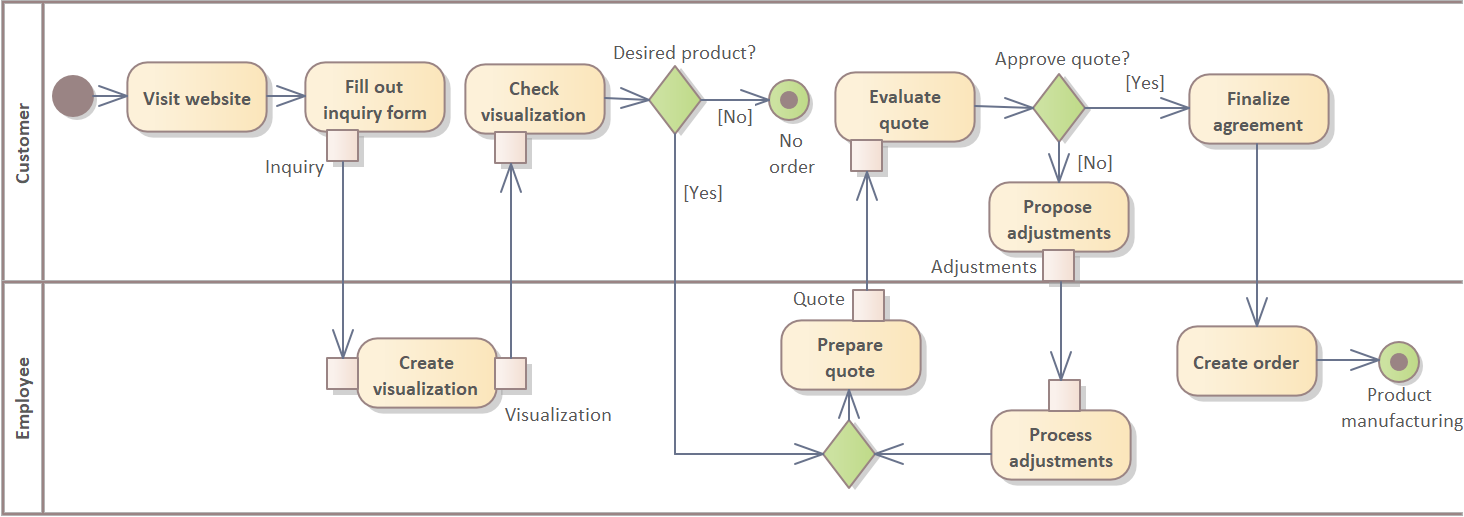
\includegraphics[width=0.67\linewidth]{images/uml_originalactivity.png}
\caption{Original order process as a UML activity diagram.}
\label{fig:uml-originalactivity}
\end{figure}
\begin{figure}[h!]
\centering
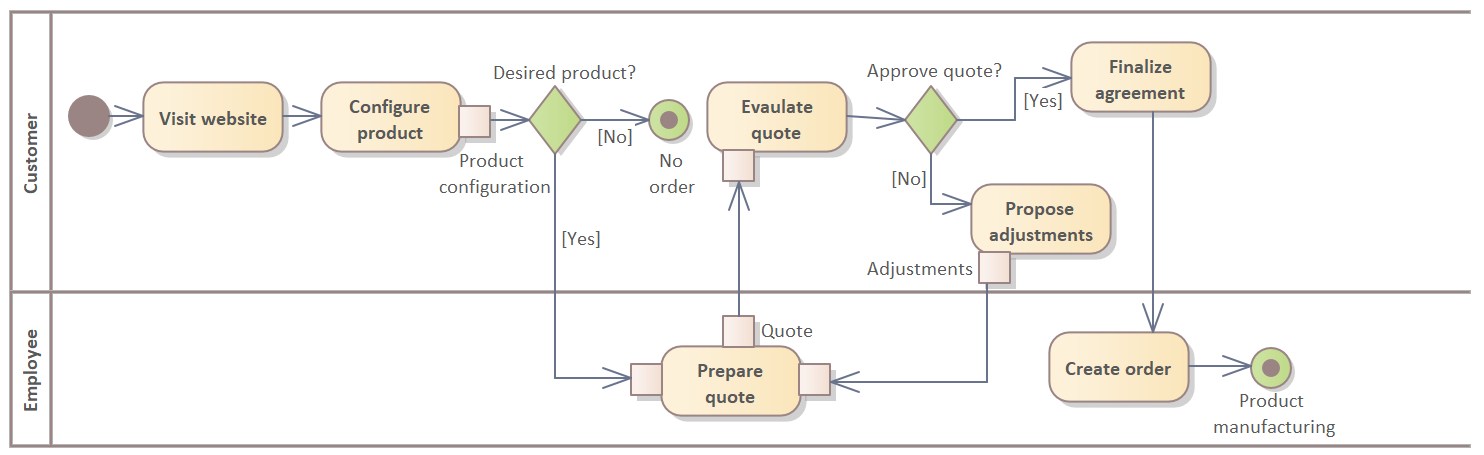
\includegraphics[width=0.67\linewidth]{images/uml_newactivity.png}
\caption{Order process with implemented solution as a UML activity diagram.}
\label{fig:uml-newactivity}
\end{figure}
\end{landscape}


%______________________________________________________________
\subsubsection{Original Process}


The UML activity diagram of the original process is illustrated in \autoref{fig:uml-originalactivity}. The inquiry and order process before deployment of the solution looks as follows. Initially, when customers wants to purchase a manufactured product, they visit the website of the company and fill out the inquiry form. Based on the information provided in the inquiry form, the employee creates a visualization, which is sent to the customer along with additional product customization informations. At this point, the customer decides if this is the product they want or if they want to stop the process there. If the customer likes the product and options presented by the employee, an iterative process begins between the customer and employee, where the employee tries to create an adequate quote for the product to the customer, while the customer sends back the proposed adjustments to the employee, who tries to process and incorporate them. When an agreement is reached, the order is placed and the product goes into production. 


%______________________________________________________________
\subsubsection{New Process}

After deploying the solution in the example company, as described in the previous sections, the inquiry and order process can change into the form illustrated in \autoref{fig:uml-newactivity}. With this change, the customer visits the company's website and directly creates the configuration of the product they desire. The steps where the employee would need to present product visualizations and options are bypassed, as these are now handled by the tool. If the customer is satisfied with the configured product, they send an inquiry containing the product configuration, and the employee can process it and base the quote on this configuration. The process then follows in the same way as in the original scenario.

This demonstrates the power of the developed tool to simplify the initial step of the process, saving the employees time that would otherwise be spent on communicating with the customer. It also allows the customers to clearly express their preferences using the tool, reducing the friction of the inquiry process and potentially leading to more conversions into orders.

The tool also finds its application in marketing, where it can be used by the company to attract more potential customers.
